\documentclass[a4paper,12pt,oneside,openany,table,xcdraw]{article}

\usepackage{setspace}
\usepackage{multirow}
\usepackage{hyperref}
\usepackage{caption}
\usepackage{indentfirst}

\usepackage[brazilian]{babel}
\usepackage[utf8x]{inputenc}
\usepackage{amsmath, graphicx, enumerate}
\usepackage{float, verbatim}
\usepackage[colorinlistoftodos]{todonotes}
\usepackage{makeidx} % Para o sumário
\usepackage{geometry}

\geometry{a4paper, hmargin={3cm, 3cm}, vmargin={3cm, 2cm} }
\setlength{\parindent}{1.0cm}

\begin{document}
\newcommand{\thedepartment}{Faculdade de Engenharia Elétrica}
\newcommand{\thecourse}{FEELT}
\newcommand{\thetitle}{FONTE DE ALIMENTAÇÃO}
\newcommand{\thetype}{Relatório da Disciplina de Circuitos Elétricos II}
\newcommand{\theproftitle}{Bacharel em Engenharia Elétrica}
\newcommand{\thestudent}{Lesly Viviane Montúfar Berrios \_ 
11811ETE001\\Ana Júlia Santana \_ 
11811ETE013}
\newcommand{\theadvisor}{Prof. Daniel Pereira de Carvalho}
\newcommand{\thecity}{Uberlândia}

\thispagestyle{empty}\newcommand*{\themonth}{\ifthenelse{\the\month < 2}{Janeiro }
                  {\ifthenelse{\the\month < 3}{Fevereiro }
                  {\ifthenelse{\the\month < 4}{Março }
                  {\ifthenelse{\the\month < 5}{Abril }
                  {\ifthenelse{\the\month < 6}{Maio }
                  {\ifthenelse{\the\month < 7}{Junho }
                  {\ifthenelse{\the\month < 8}{Julho }
                  {\ifthenelse{\the\month < 9}{Agosto }
                  {\ifthenelse{\the\month < 10}{Setembro }
                  {\ifthenelse{\the\month < 11}{Outubro }
                  {\ifthenelse{\the\month < 12}{Novembro }{Dezembro }}}}}}}}}}}}
                  
\begin{titlepage}
\begin{center}

	\vspace{-0.5cm}

  \begin{figure}[hbt!]
		\begin{center}
		   
\includegraphics[width=2.8cm]{ufu-logo.png}
		\end{center}
	\end{figure}
 	%\vspace{-4cm}

%\begin{doublespacing}

  \Large{\textbf{Universidade Federal de Uberlândia}}\\
  \large{\thedepartment}\\
  \large{\thecourse}\\


\vspace{5.8cm}
  \par
  \large\textbf{\thetitle}
\vspace{5.8cm} 

%\end{doublespacing}
  \par
  \thetype\\
  por\\
  %\hspace{2cm}\large{}\\

\vspace{0.8cm}
\par
  \normalsize{\thestudent}\\ [2cm]
  \theadvisor

\par\vfill
  \thecity, \themonth / \the\year

\end{center}

\end{titlepage}

%% Comeca o documento !

\onehalfspacing
\tableofcontents % sumário
\newpage

\section{Introdução}
Um circuito
% A importancia da fonte

\section{Planejamento} % e simulações
Nesta seção, é apresentado as primeiras considerações para a realização do projeto, desde a análise do circuito base por meio de simulações, até à escolha dos componentes a serem utilizados na confecção do circuito impresso.

\subsection{Circuito esquemático}
A Figura \ref{circuito} mostra o circuito no qual este projeto de baseará.

\begin{figure}[H]
\centering
\captionsetup{font=scriptsize}
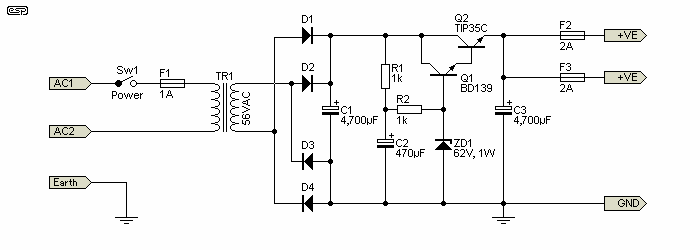
\includegraphics[width=16cm]{fonte}
\caption{Circuito da fonte de alimentação \cite{amp}.}
\label{circuito}
\end{figure}

\subsection{Componentes}
\subsection{Orçamento}

\section{Simulação}
%MULTSIM tbm pode ser


\section{Funcionamento do circuito}


\subsection{Retificação}
Esta etapa transforma a tensão alternada em uma tensão contínua pulsante

\subsection{Filtragem}
transforma a tensão contínua pulsante em uma tensão contínua quase perfeita. Mas essa tensão contínua apresenta, quando a fonte é ligada a uma carga, uma oscilação chamada Tensão de Ripple. Para eliminar esse fator incômodo existe ainda outra etapa...

\subsection{Regulação}
Esta última etapa tem por objetivo eliminar por completo a tensão de oscilação.  É claro que não elimina totalmente, mas remove boa parte. Esta última etapa pode consistir em regulação com diodo zener, com emissor zener, existem também alguns circuitos com transistores e, por último, reguladores em CI, como a família 78XX para tensões positivas e 79XX para tensões negativas.


\section{Memória de Cálculo}

\newpage
\begin{thebibliography}{9} 

\bibitem{amp}
    Rod Elliott,
    “El Cheapo - A Really Simple Power Amplifier”, ESP, Elliott Sound Products, 2005.
 Disponível em:
 \url{https://sound-au.com/project12a.htm}. Acesso em: out. 2019.

\end{thebibliography}
\end{document}
